\documentclass[a4paper,11pt,french]{article}

    \usepackage[utf8]{inputenc}
    
    \usepackage{mathrsfs}
    \usepackage[english]{babel}
    \usepackage{mathtools} % includes amsmath
    \usepackage{amssymb}
    \usepackage{amsthm}
    \usepackage{amscd}
    \usepackage{todonotes}
    
    \usepackage{multirow}
    \usepackage{enumerate}
    
    \usepackage{tikz}
    \usepackage{framed}
    \usepackage[colorlinks]{hyperref}
    \usepackage[T1]{fontenc}
    
  
    
    \title{Discrete Optimization: Homework \#12, Ex. \#4}
    \author{Denis Steffen, Yann Eberhard \& Gaëtan Bossy}
    
    \begin{document}
    
    \maketitle
Given a graph $G=(V=\{v_1,...,v_n\},E)$, we can obtain an associated bipartite graph $G'=(V',E')$ with $V'=A\cup B$, $A=\{a_i : i\in \{1,...,n\}\}$ and $B=\{ b_j  : j \in \{1,...,n\}\}$, $(a_i,b_j)\in E'$ if and only if $(v_i,v_j)\in E$. Then one can find a 2-matching in $G$ if and only if one can find a perfect matching in $G'$, which can be done in polynomial time. If $M'$ is a perfect matching of $G'$, then $\forall e\in M'$, $e=(a_i,b_j)$ or $e=(b_j,a_i)$ and we can add $(v_i,v_j)$ to the 2-Matching $M$ in $G$.\\

By König-Hall's Theorem, we can only find a perfect matching in $G'$ if $|N(S)|\geq|S|\quad \forall S\subseteq A$.

\begin{center}

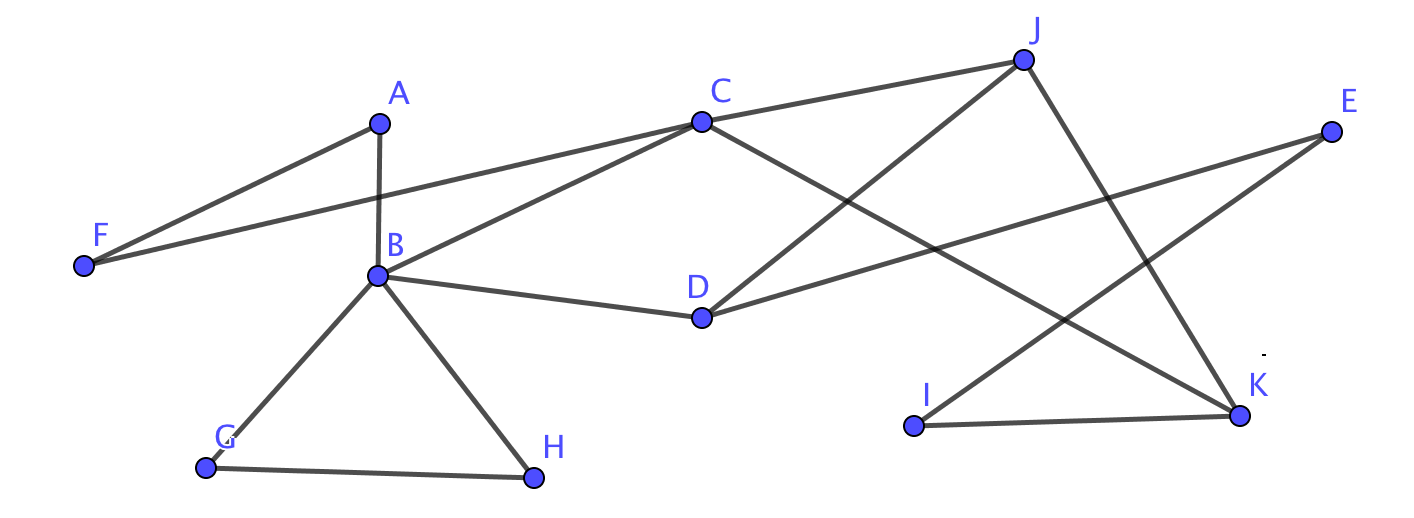
\includegraphics[scale=0.3]{Graph} 

\end{center}
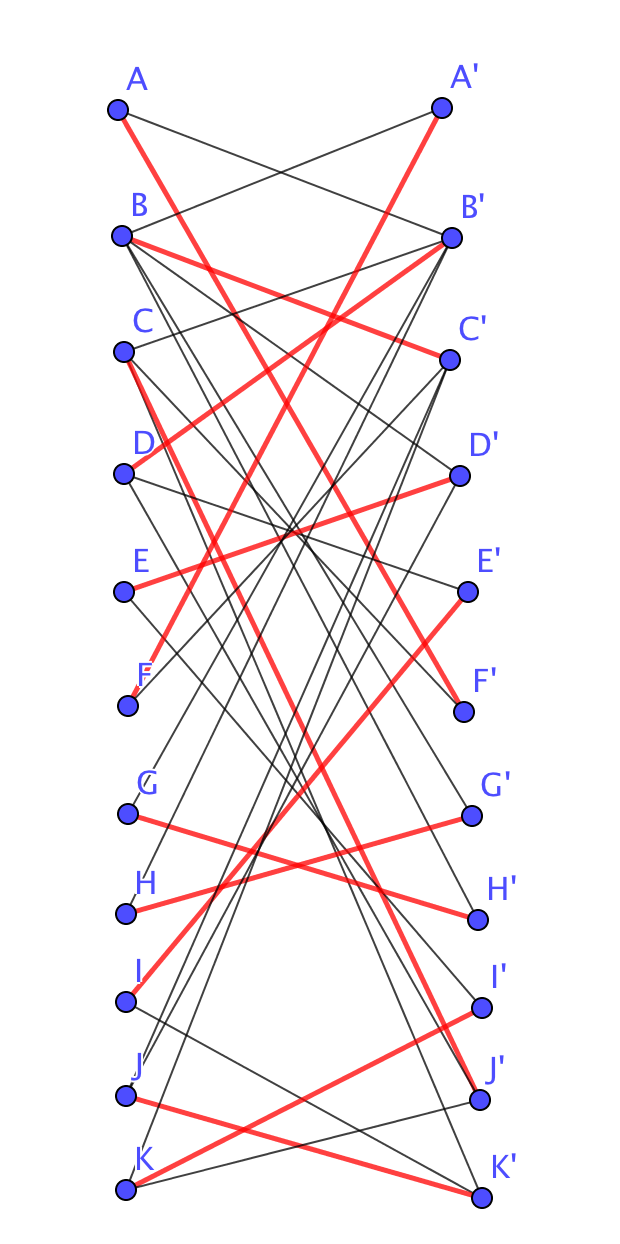
\includegraphics[scale=0.3]{Bipartite} \hfill 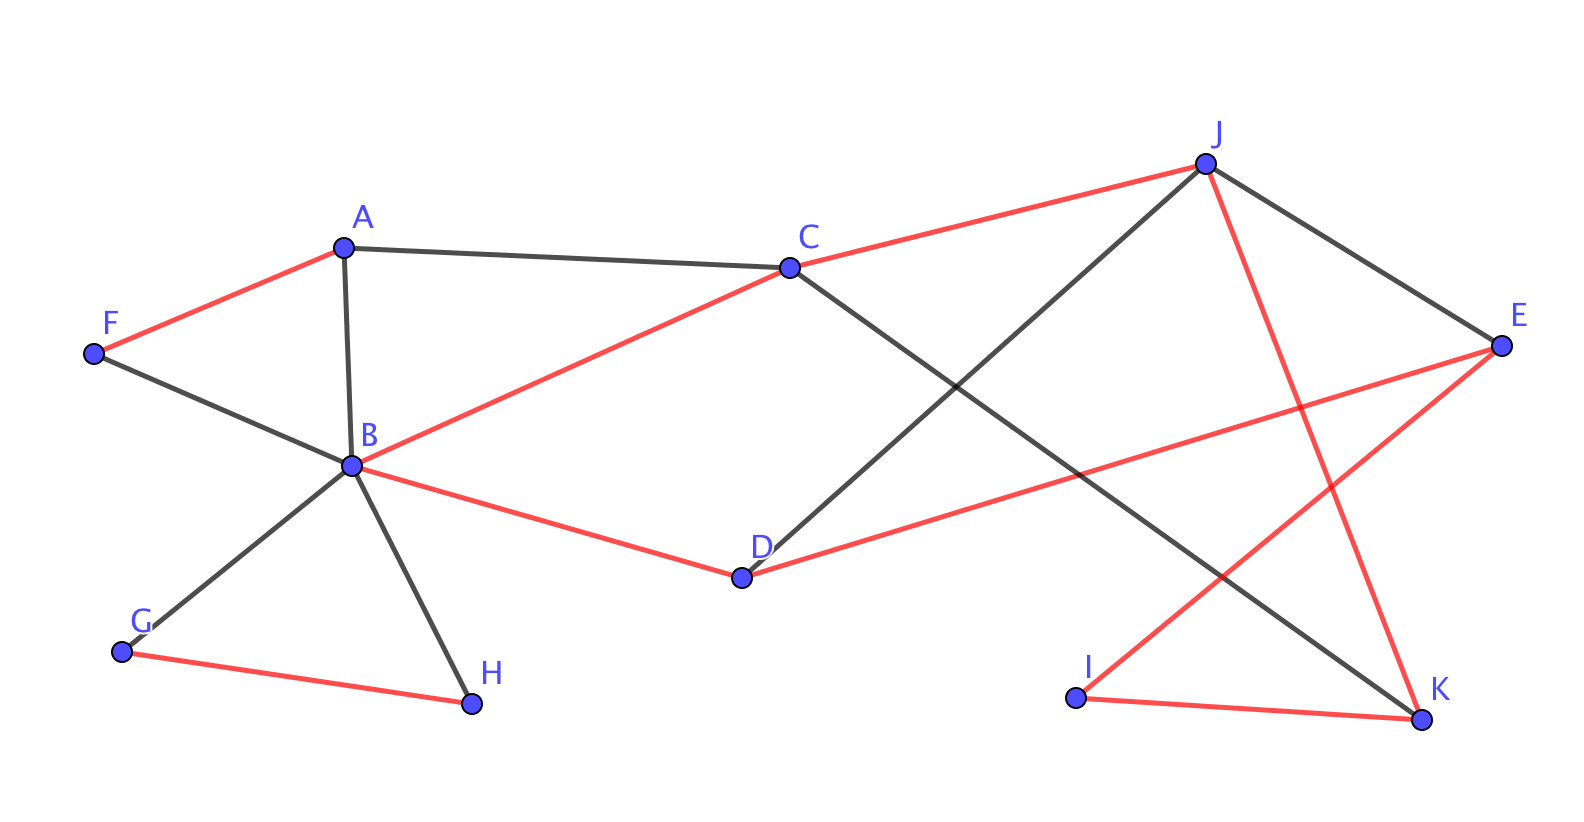
\includegraphics[scale=0.3]{2-matching} 



Now, we need to prove that : 
\begin{center}
There is a 2-matching in $G \Leftrightarrow$ there is a perfect matching in $G'$
\end{center}

$\Leftarrow$) : Suppose $G'$ has a perfect matching $M'$, for all $(a_i,b_j) \in M'$ we put $(v_i,v_j)$ in $A$. It is impossible that we have $i=j$ by construction of $G'$. We can suppose without loss of generality that there doesn't exist $a_i,b_j$ and $a_j,b_i$ in $M'$ for all $i \neq j$, because if there is one we can put $(v_i,v_j)$ in $A$ and consider only the other edges of $M'$. Now, we suppose that there doesn't exist such thing in $M'$. Every vertex $v_i$ is an endpoint of exactly two edges in $A$ because there exist only $(a_i,b_j)$, $(a_k,b_i) \in M'$. Since $M'$ is a perfect matching, all vertices of $G$ are the endpoint of exactly two edges of $A$, this implies that all edges of $A$ make cycles and so $A$ is a 2-matching.\\\\

$\Rightarrow$) : Suppose that there exists a 2-matching $A$ in $G$. Without loss of generality, we can suppose that the matching consists in only one cycle. If there are more, we can repeat the process for each cycle. Suppose the 2-matching makes only one cycle. We can direct the cycle to make it a directed cycle and create $A'$ that is $A$ with the directed edges. Now, we define $M' := \{ (uv) | (uv) \in A' \}$. We need to show that $M'$ is a perfect matching in $G'$. For every vertices $a_i\in A$ there exists $b_j\in B$ such that $(a_i,b_j) \in M'$ because there exists an $v_j \in G$ s.t. $(v_i,v_j) \in A'$. Without loss of generality, we can suppose that there is only one cycle because we can repeat the process for each cycle. So now we suppose that there is only one cycle. For each vertex $v_i \in G$ there exists only one edge $(v_i,v_j) \in A'$ coming from $v_i$ and only one $(v_k,v_i) \in A'$ going to $v_i$. This implies that every vertex in $G'$ is only touched by one edge from $M'$.
$\qed$



  \end{document}
